
\section{Problem Analysis}
\begin{frame}{Problem Analysis}{Camera Limitations}
\begin{columns}
    \column{0.5\textwidth}
\begin{block}{}
    \visible<1->{
    Spatial resolution - Pixel density
    \begin{itemize}
        \item Image sensor
        \item Optical lens
        \item Lossy compression algorithms
        \item Blur \& noise
    \end{itemize}
}
\visible<2->{
\begin{figure}[!htb]
\minipage{0.5\textwidth}
\includegraphics[width=0.9\linewidth]{../../Figs/Introduction/blur.jpg}
  \caption*{Blurred}
  \endminipage\hfill
\minipage{0.5\textwidth}
  \includegraphics[width=0.9\linewidth]{../../Figs/Introduction/noise.png}
  \caption*{Noisy}
\endminipage
\end{figure}
}
\end{block}

\column{0.5\textwidth}
\begin{block}{}
    \visible<3->{
\begin{figure}
    \includegraphics[width=0.5\linewidth]{../../Figs/Techanal/resLow.tex}
        \caption*{Low resolution}
 \end{figure}
 \begin{figure}
    \includegraphics[width=0.5\linewidth]{../../Figs/Techanal/resHigh.tex}
        \caption*{High resolution}
\end{figure}
}
\end{block}
\end{columns}
\end{frame}

\begin{frame}{Problem Analysis}{Super-Resolution}
    \begin{columns}
        \column{0.5\textwidth}
        \begin{block}{}
            \visible<1->{
            From low resolution to high resolution
            \begin{itemize}
                \item Single image - Hallucination
                    \begin{itemize}
                        \item Learn the relationship
                    \end{itemize}
            \end{itemize}
            \begin{itemize}    
                \item Multiple images - Reconstruction
                    \begin{itemize}
                        \item Imaging model
                    \end{itemize}

            \end{itemize}
        }
        \end{block}
            \column{0.5\textwidth}
            \begin{block}{}
                \visible<2->{
 \begin{figure}[!htb]
    \minipage{0.4\textwidth}
        \includegraphics[width=\linewidth]{../../Figs/Introduction/butterfly_low.jpg}
            \caption*{LR}
    \endminipage\hfill
    \minipage{0.4\textwidth}%
        \includegraphics[width=\linewidth]{../../Figs/Introduction/butterfly_high.jpg}
            \caption*{HR}
    \endminipage
\end{figure}}



            \end{block}
        \end{columns}
        \begin{block}{}

        \begin{figure}[!htb]
            \visible<3->{
    \minipage{0.15\textwidth}
        \includegraphics[width=\linewidth]{../../Figs/Techanal/modelOrg.jpg}
            \caption*{Original}
        \endminipage\hfill}
        \visible<4->{
    \minipage{0.15\textwidth}
        \includegraphics[width=\linewidth]{../../Figs/Techanal/modelWarp.jpg}
            \caption*{Warped}
        \endminipage\hfill}
        \visible<5->{
    \minipage{0.15\textwidth}%
        \includegraphics[width=\linewidth]{../../Figs/Techanal/modelBlur.jpg}
            \caption*{Blurred}
        \endminipage\hfill}
        \visible<6->{
    \minipage{0.15\textwidth}%
        \includegraphics[width=\linewidth]{../../Figs/Techanal/modelD.jpg}
            \caption*{Low res}
        \endminipage\hfill}
        \visible<7->{
    \minipage{0.15\textwidth}%
        \includegraphics[width=\linewidth]{../../Figs/Techanal/modelNoise.jpg}
            \caption*{Noisy}
        \endminipage}
        \caption*{Imaging Model}
\end{figure}
\end{block}
\end{frame}

\begin{frame}{Problem Analysis}{Deep Learning}
    \begin{block}{}
        Current state of the art
        \begin{itemize}
            \item Patch extract $\rightarrow$ Non-linear mapping $\rightarrow$ Reconstruct patches
        \end{itemize}
        \begin{figure}
            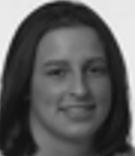
\includegraphics[width=0.7\linewidth]{figs/srcnn.png}
            \caption*{Super-Resolution CNN \footnote{Chao Dong, C. C. Loy, Kaiming He and Xiaoou Tang 2016, "Image Super-Resolution Using Deep Convolutional Networks"}}
        \end{figure}
    \end{block}
\end{frame}

\begin{frame}{Problem Analysis}{Deep Learning}
    \begin{block}{}
       % \setlength{\abovecaptionskip}{-2ex}
        \setlength{\belowcaptionskip}{-2ex}
\begin{figure}
    \vspace*{-1cm}
    \includegraphics[width=0.32\linewidth]{figs/rec_cnn.png}
    \caption*{Ground truth, SRCNN, DRCN \footnote{Jiwon Kim, Jung Kwon Lee and Kyoung Mu Lee 2015, "Deeply-Recursive Convolutional Network for Image Super-Resolution}}
\end{figure}
\begin{figure}
    \includegraphics[width=0.35\linewidth]{figs/bi.png}
    \caption*{Ground truth, CNN, Bi-channel CNN \footnote{Jiwoin Zhou, Haoqiang Fan, Zhimin Cao, Yuning Jiang, and Qi Yin. 2015, "Learning face hallucination in the wild"}}
\end{figure}
%\setlength{\abovecaptionskip}{0ex}
\setlength{\belowcaptionskip}{2ex} 
    \end{block}
\end{frame}

\begin{frame}{Problem Analysis}
    Problem Statement
    \begin{itemize}
        \item Can a SR algorithm consisting of both a classic SR and a deep-based SR method be used to increase the image quality of surveillance video?
    \end{itemize}
\end{frame}


